%-------------------------------------------------------------------------------
% This is a template ATLAS Paper that contains suggestions and hints on how
% to get your paper draft into a form that minimises the amount of work needed
% to get it approved by the collaboration - assuming that the physics is OK!
%-------------------------------------------------------------------------------
\documentclass[UKenglish]{latex/atlasdoc}

% Use listings package and make it look like verbatim
\usepackage{listings}
\lstset{
  basicstyle=\ttfamily,
  columns=fullflexible,
  keepspaces=true,
}

% Standard packages that can and should be used in ATLAS papers
% Use biblatex and biber for the bibliography
\usepackage[biblatex]{latex/atlaspackage}
% Useful macros
\usepackage{latex/atlasphysics}
\usepackage{tikz}

% Files with references in BibTeX format
\usepackage{latex/atlas-biblatex}
\addbibresource{BayesianNote.bib}
\addbibresource{./bibtex/bib/BayesianNote.bib}
\addbibresource{../atlas-latex.bib}

% Paths for figures
\graphicspath{{./logos/},{figures/}}

\newcommand{\Macro}[1]{\texttt{\textbackslash #1}\xspace}
\newcommand{\Option}[1]{\textsf{#1}\xspace}
\newcommand{\Package}[1]{\texttt{#1}\xspace}

%-------------------------------------------------------------------------------
% Generic document information
%-------------------------------------------------------------------------------

% Set author and title for the PDF file
\hypersetup{pdftitle={ATLAS paper template},pdfauthor={ATLAS Publications Committee}}

\AtlasTitle{Statistical analysis tool used in the ATLAS dijet resonance search}

\author{Lydia Beresford, Katherine Pachal}
%-------------------------------------------------------------------------------
%\subsection{Author list}
%\label{sec:author}
%-------------------------------------------------------------------------------

%The author list will be provided by the Authorship Committee and Physics Office. It will be created by the Physics Office at the time of the first draft announcement by PubCom, and added to the CDS record for the paper as a separate document from the paper itself.Requests for exceptional authorship or for removal of names should be made to the Spokesperson and Authorship Committee while the first draft is circulating.The author list will be archived when the second draft announcement is made by Publication Committee, and again added to the CDS record as a separate document from the paper. The front page of the paper should name ``The ATLAS Collaboration'' as the author.

%\AtlasVersion{1.0}

\AtlasAbstract{%
This note describes the the statistical analysis tool which is used in the 2015 dijet resonance search with $\sqrt{s} = \SI{13}{\TeV}$ data.  The tool includes a frequentist `search phase' which fits a function to the dijet invariant mass distribution and uses the BumpHunter \textcolor{red}{reference} algorithm to search for, and quantify, any local excesses. %or steeply falling backgrounds
If no significant excess is observed %ask defn of significant?
 then the `limit setting phase' is performed. In this phase a bayesian approach is used to set limits on New Phenomena using code based on the Bayesian Analysis Toolkit (BAT) \textcolor{red}{reference}.  % say somewhere runs on lxplus?

 % This document was generated using version \ATPackageVersion\ of the ATLAS \LaTeX\ package.
}

%-------------------------------------------------------------------------------
% Extra definitions - it is usually better to collect these in a separate file
%-------------------------------------------------------------------------------
% Shorthand for \phantom to use in tables
\newcommand*{\pho}{\phantom{0}}
\newcommand{\BibTeX}{\textsc{Bib\TeX}}


%-------------------------------------------------------------------------------
% This is where the document really begins
%-------------------------------------------------------------------------------
\begin{document}

\tableofcontents
\clearpage

%-------------------------------------------------------------------------------
\section{Introduction to the package structure and order of running}
\label{sec:intro}
%-------------------------------------------------------------------------------

The structure of the StatisticalAnalysis package is displayed in Figure~\ref{fig:StatsStructure}, along with the additional packages that it requires. 

\begin{figure}[htbp]
  \centering
  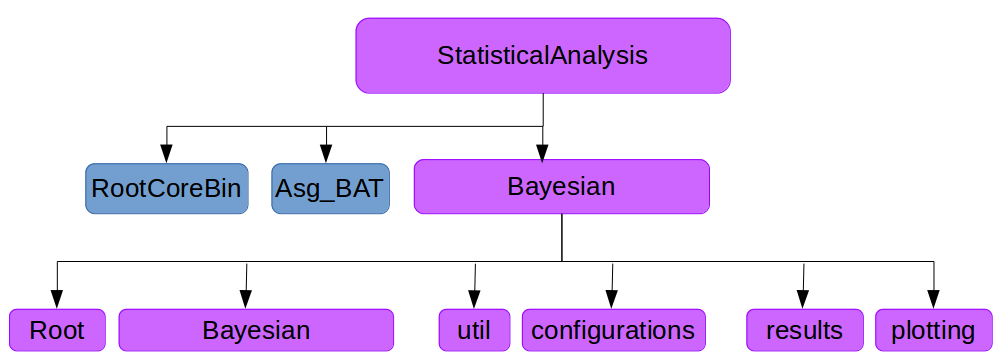
\includegraphics[width=\columnwidth]{StatsStructurev1}
  \caption{The structure of the StatisticalAnalysis package is displayed (purple boxes), along with the additional packages that it requires (blue boxes).}
  \label{fig:StatsStructure}
\end{figure}

Within the \verb Bayesian  directory, the \verb util  directory contains the following C++ source files:
\begin{itemize}
  \item SearchPhase.cxx
  \item SetLimitsOneMassPoint.cxx
  \item LimitSettingPhase.cxx
 \item doGaussianLimits.cxx
\end{itemize}
These are the main files that perform the statistical analysis and they are run in the order shown above. Their corresponding configuration files are stored in the \verb configurations  folder. The supporting C++ source code containing the classes and functions used in main files are in the \verb Root  folder with their own header files stored in the \verb Bayesian  folder. When the main files are run their outputs are stored in the \verb results  folder, and these outputs are used to make more meaningful plots using the \verb plotting    package, which is written in python. 

Section~\ref{sec:quickstart} explains how to download the StatisticalAnalysis package and also how to run it and plot the results. An explanation of each of the main source files is provided in  section~\ref{sec:searchexpl} (search phase) and in section~\ref{sec:limitexpl} (limit setting phase), these sections can be skipped if you are familiar with the package. Section ~\ref{sec:lhcpplots} shows examples of the plots that are produced when following the quick start guide. Section ~\ref{sec:mistakes} gives common mistakes and the solutions to them. Section ~\ref{sec:examplessearch} and section ~\ref{sec:exampleslimit} provide examples of common modifications that can be made to the code for the search phase and limit setting phase, respectively.  

%-------------------------------------------------------------------------------
\section{Quick start guide to downloading and running }
\label{sec:quickstart}
%-------------------------------------------------------------------------------
A quick start guide is presented to explain how to download and setup the code. How to run the search phase is outlined in section~\ref{subsec:search} and how to run the limit setting phase is outlined in section ~\ref{subsec:limit}. 
\\\\\textbf{Some commands span more than one line due to text wrapping, if lines following initial command are indented then they belong to the initial command and any extraspaces should be removed when copying the command.}
\begin{description}

\item Instructions for setting up the code for the \textbf{ first time}:\\

  \item[Step 1] Starting in a directory of your choice, make a directory for the statistical analysis and enter this directory:
\begin{lstlisting}[breaklines]
mkdir StatisticalAnalysis
cd StatisticalAnalysis
\end{lstlisting}

  \item[Step 2] Set-up ATLAS environment:
\begin{lstlisting}[breaklines]
setupATLAS
\end{lstlisting}
%rcSetup Base,2.0.26

  \item[Step 3]  Obtain setup script:
\begin{lstlisting}[breaklines]
svn export svn+ssh://svn.cern.ch/reps/atlasphys-exo/Physics/Exotic/JDM/DiJet/StatisticalAnalysis/Bayesian/trunk/scripts/setup-StatisticalAnalysis.sh
\end{lstlisting}

  \item[Step 4]  Source setup script:
\begin{lstlisting}[breaklines]
source setup-StatisticalAnalysis.sh
\end{lstlisting}

%\item[Step 2] Check out the Bayesian package from SVN using the following command : 
%\begin{verbatim}svn co svn+ssh://svn.cern.ch/reps/atlasphys-exo/Physics/Exotic/JDM/DiJet/
%StatisticalAnalysis/Bayesian/trunk/ Bayesian\end{verbatim} 

%\item[Step 3] Setup the ATLAS software environment, then setup an Analysis Release as follows:
%\textcolor{red}{Give link to latest version/software tutorial and tell how unset and re-set?}
%\begin{verbatim}setupATLAS
%rcSetup Base,2.0.26\end{verbatim}

%\item[Step 3] Check out  Asg\_BAT  \textcolor{red}{reference }, and then 'find all packages' and compile using the following commands : 
%\begin{verbatim}rc checkout_pkg atlasoff/AsgExternal/Asg_BAT/tags/Asg_BAT-00-00-02
%rc find_packages 
%rc compile
%\end{verbatim}

 %\item[Step 4] Set up the python path as follows:
%\begin{verbatim} cd Bayesian
%. Setup.sh
%\end{verbatim}

\item[Step 5] Inputs (read all of this step before downloading inputs):

\vspace{0.2cm}
The code requires:
\begin{itemize}
\item A data (or MC) background $m_{jj}$ distribution
\item Signal MC $m_{jj}$ distributions 
\item Theory lines (for plotting)
\item Signal templates (for plotting)
\end{itemize}
If you are re-producing the LHCP conference version of the analysis then the LHCP inputs are located in:
\begin{lstlisting}[breaklines]
eos/atlas/atlascerngroupdisk/phys-exotics/jdm/dijet/statsinputs/RunII/LHCP/inputs/
\end{lstlisting}

This directory should be copied to your local \verb Bayesian  directory, retaining the name \verb inputs . The contents of \verb inputs  directory is as follows:
\begin{itemize}
\item \verb Data_fGRL_Hopeful_20150828  (Contains: data background  $m_{jj}$ distribution) 
\item \verb Full_25ns_20150813/BlackMax/StatisticalHists/1fb  (Contains: Quantum Black Hole MC $m_{jj}$ distributions) 
\item \verb Full_25ns_20150813/QStar/StatisticalHists/1fb   (Contains: Excited quark MC $m_{jj}$ distributions)  
\item \verb xsecandacceptance  (Contains:  Theory line and signal templates)  
\item \verb Full_25ns_20150813/QBH/StatisticalHists/1fb  (Contains: Quantum Black Hole QBH generator AFII MC $m_{jj}$ distributions \textbf{Not needed to reproduce the LHCP version of the analysis})
\item \verb Full_25ns_20150813/QBH_FullSim/StatisticalHists/1fb  (Contains: Quantum Black Hole QBH generator full sim MC $m_{jj}$ distributions \textbf{Not needed to reproduce the LHCP version of the analysis})

\end{itemize}

If using other inputs i.e. non-LHCP then the usual procedure is to:\\ Make a directory in the Bayesian package to store your inputs (if it doesn't exist already):
\begin{lstlisting}[breaklines]
cd Bayesian
mkdir inputs
\end{lstlisting}

The data and MC inputs can be found in the following directory: 
\begin{lstlisting}[breaklines]
/eos/atlas/atlascerngroupdisk/phys-exotics/jdm/dijet/inputs/
\end{lstlisting} or produced by the user. Note that histograms are required as inputs, NOT trees, so it is not necessary to copy across any \verb tree  directories. The corresponding theory and signal templates can be found in the 
\begin{lstlisting}[breaklines]
eos/atlas/atlascerngroupdisk/phys-exotics/jdm/dijet/statsinputs/RunII/inputs/
\end{lstlisting} directory, or produced by the user.


% TEMPORARY The inputs which are currently being used for the code can be found in \verb /afs/cern.ch/work/l/lberesfo/public/forDijets/inputs the inputs folder should be copied to the \verb StatisticalAnalysis/Bayesian folder in your downloaded copy of the package and the folder should keep the name inputs. \textcolor{red}{Fill in more once file format settled, as currently have to hadd together files to make inputs of right form for JES uncertainty}
% These inputs include the dijet invariant mass histogram, Beam uncertainty histograms, PDF uncertainty histograms, \textcolor{red}{resolution y cut} and JES matrices for signal samples \textcolor{red}{more}:
%\begin{verbatim}mkdir Data\end{verbatim}
%\begin{verbatim}cd Data\end{verbatim}
%\begin{verbatim}mkdir inputs\end{verbatim}
%\begin{verbatim}source /afs/cern.ch/project/eos/installation/atlas/etc/setup.sh\end{verbatim} 
%\begin{verbatim}eos cp -r root://eosatlas//eos/atlas/atlascerngroupdisk/phys-exotics/jdm/dijet/sta
%tsinputs/ inputs/\end{verbatim}
%\textbf{Close this shell and open a new one as this one is still linked to eos!}
%\\For more information about the inputs to the code that are provided, see appendix ~\ref{app:inputs}. These inputs are the ones that were used in the 2012 $ \SI{8}{\TeV}$  dijet resonance search, and they are included as an example. \textcolor{red}{give links/expl in appendix A how made/format of inputs?}

\item Instructions for setting up the code each \textbf{subsequent time}: 

\item[Step 1] Setup the package and execute it whenever you log in:
\begin{lstlisting}[breaklines]
cd StatisticalAnalysis
setupATLAS
rcSetup
rc compile
cd Bayesian
. Setup.sh
\end{lstlisting}
The code should be compiled before running whenever changes to source files or to header files have been made.
\end{description}

%-------------------------------------------------------------------------------
\subsection{Performing the search phase}
\label{subsec:search}
%-------------------------------------------------------------------------------
Performing the search phase involves running \verb SearchPhase.cxx, which takes the dijet invariant mass histogram as an input. The \verb Run_SearchPhase.py  script is used in order to run  \verb SearchPhase.cxx  in the util directory which uses the configuration file \verb Step1_SearchPhase.config  in the configurations directory. The script creates results,  plots and log files directories for you and puts all code outputs into the relevant folders in a sub-directory with a name of your choice (specified by folderextension in \verb Run_SearchPhase.py ). 
\begin{description}
\item [Step 1] The user should modify the fields in the \verb ***** User specifies *****  section of \verb Run_SearchPhase.py  to suit their inputs and requirements (Currently set-up to re-produce LHCP result). 

\item [Step 2] If necessary, the user should modify any fields in \verb Step1_SearchPhase.config  that are not over-written by \verb Run_SearchPhase.py , any fields that are over-written are labelled in the configuration file, e.g. fit function starting parameters (Currently set-up to re-produce LHCP result).

\item [Step 3] Run the script as follows:
\begin{lstlisting}[breaklines]
python Run_SearchPhase.py
\end{lstlisting}
Results can be found in: \verb results/Step1_SearchPhase/folderextension  where 
\verb plotextension  is a name specified by the user in the \verb Run_SearchPhase.py  script. Plots are stored in the\\ 
\verb plotting/SearchPhase/plots/folderextension .  For examples of some of the plots that should be produced, see section ~\ref{subsec:spplots}, these can be compared to the plots that you've just obtained.

\paragraph{}\textbf{Note}: To change the ATLAS label displayed on the plots (e.g. Internal, Preliminary, etc.), modify the number in the following line \verb myPainter.setLabelType(2)  in \\\verb plotting/SearchPhase/plotSearchPhase.py , and re-run \verb Run_SearchPhase.py  with only  \verb doPlotting set to true.

\paragraph{}\textbf{Aside}: To run the search phase manually the following commands can be used:
\begin{lstlisting}[breaklines]
SearchPhase --config configurations/Step1_SearchPhase.config
python plotting/SearchPhase/plotSearchPhase.py
\end{lstlisting}
\end{description}


%. This file can be changed if necessary and an annotated version of this configuration file is included in appendix ~\ref{app:searchconfig} to explain what each quantity is and to give sensible values for testing out the package.
% The values used in the paper are included as comments in the code and should be used in order to reproduce the paper results, for further information about this see section ~\ref{subsec:fullpaper}.\textbf{Please note} that the range and initial fit function parameters may need to be changed when running the search phase on a different mass spectrum to the one provided, e.g. a 13 TeV mass spectrum, for information about selecting the correct range and initial fit function parameters consult section ~\ref{subsec:chooseparam}.

%  \item[Step 2] Run the search phase, specifying the name of the configuration file you would like to use:
%\begin{verbatim}cd Bayesian\end{verbatim}
%\begin{verbatim}SearchPhase --config configurations/SearchPhase.config\end{verbatim}
%\textcolor{red}{mention values etc code gives/what printed out?}
%  \item[Step 3] Obtain \verb SearchPhase_results.root  in the \verb results  folder. See appendix ~\ref{app:searchresults} for an explanation of each plot in \verb SearchPhase_results.root .

%\item [Step 4] In order to combine plots in \verb SearchPhase_results.root  into more meaningful plots \verb plotter.py  in the \verb plotting/myplots  directory is used. To produce the plots do the following: 

%\begin{verbatim}cd plotting/myplots\end{verbatim}

%\begin{verbatim}python plotter.py -b\end{verbatim}
%\end{description}
%An explanation about the aims of the search phase, the stages that are involved, and examples and interpretations of the output plots is presented in section ~\ref{sec:searchexpl}.

%-------------------------------------------------------------------------------
\subsection{Performing the limit setting phase }
\label{subsec:limit}
%-------------------------------------------------------------------------------
Running the limit setting phase for models involves first running \verb setLimitsOneMassPoint.cxx  and then \verb LimitSettingPhase.cxx. %To set limits on generic Gaussians or \textcolor{red}{Breit-Wigner} distributions then \verb doGaussianLimits.cxx  is run. 
\verb setLimitsOneMassPoint.cxx  takes the output root file from the search phase as an input, along with histograms of the nominal and JES shifted signal MC mjj spectra, for each mass point. The outputs of \verb setLimitsOneMassPoint.cxx  are a root file for each mass point. The single mass points are then scaled by luminosity and graphed in \verb LimitSettingPhase.cxx. %\textcolor{red}{ divide points by luminosity and graph them}.

\paragraph{}  The \verb Run_Limits.py  script is used in order to run  
\verb setLimitsOneMassPoint.cxx  in the util directory which uses the configuration file
 \verb Step2_setLimitsOneMassPoint_QStar.config , for example, in the configurations directory, and to run LimitSettingPhase.cxx in the util directory which uses the configuration file 
\verb Step3_LimitSettingPhase_QStar.config , for example,  in the configurations directory.  The script creates  results,  plots and log files directories for you and puts all code outputs into the relevant folders in a sub-directory with a name of your choice (specified by plotextension in
\verb Run_Limits.py ).

\begin{description}
\item [Step 1] The user should modify the fields in the \verb ***** User specifies *****  section of \verb Run_Limits.py  to suit their inputs and requirements (Currently set-up to re-produce LHCP result). 

\item [Step 2] If necessary, the user should modify any fields in \verb Step2_setLimitsOneMassPoint_XXX.config  and \verb Step3_LimitSettingPhase_XXX.config  (where XXX is the signal Model) that are not over-written by \verb Run_Limits.py, any fields that are over-written are labelled in the configuration files (Currently set-up to re-produce LHCP result). 

\item [Step 3] Run the script as follows:
\begin{lstlisting}[breaklines]
python Run_Limits.py
\end{lstlisting}

The first time the script is run, only \verb dosetLimitsOneMassPoint  should be set to True and \verb doLimitSettingPhase  and \verb doPlotting  are set to False, such that only \verb setLimitsOneMassPoint.cxx  is run. \paragraph{}
\textbf{This step should be run for each signal you are setting limits on!}  \paragraph{} To re-produce the LHCP result, run once with the `QBH BlackMax' part in  the \verb Signal  \verb information  section uncommented, then comment this part out and uncomment the `QStar'  part and re-run. Once all batch jobs are completed then  \verb dosetLimitsOneMassPoint   should be set to False, \verb doLimitSettingPhase  and \verb doPlotting  are set to True, such that only \verb LimitSettingPhase.cxx  and \verb plotLimitSetting.py  are run, and again this is run twice, once for each signal type. Note that the limit value and bump low edge and high edge are printed out during the plotting and are displayed under `Easy to find paper Values' in the plotting output. 

\paragraph{}Results can be found in: \verb results/Step2_setLimitsOneMassPoint /plotextension  and \\\verb results/Step3_LimitSettingPhase/plotextension  where \verb plotextension  is a name specified by the user in the \verb Run_Limits.py  script. Plots are stored in the \\\verb plotting/LimitSettingPhase/plots/plotextension  and all Log files are stored in\\\verb StatisticalAnalysis/LogFiles/plotextension . For examples of some of the plots that should be produced, see section ~\ref{subsec:limplots}, these can be compared to the plots that you've just obtained, also the limit values and bump low and high edge values are provided for comparison. 

\paragraph{}\textbf{Note}: To change the ATLAS label displayed on the plots (e.g. Internal, Preliminary, etc.), modify the number in the following line \verb myPainter.setLabelType(2)  in \\\verb plotting/LimitSettingPhase/plotLimitSetting.py , and re-run \verb Run_Limits.py with only  \verb doPlotting set to true for each signal type.


\paragraph{}\textbf{Aside}: To run the limit setting manually the following commands can be used:

\begin{lstlisting}[breaklines]
setLimitsOneMassPoint --config configurations/Step2_LimitSettingPhase_QStar.config --mass 4500

LimitSettingPhase --config configurations/LimitSetting/Step3_LimitSettingPhase.config

python plotLimitSetting.py

\end{lstlisting}

\end{description}

%-------------------------------------------------------------------------------
\section{LHCP plots for comparison}
\label{sec:lhcpplots}
%-------------------------------------------------------------------------------

Examples of the plots and values that should be produced when following the above instructions are shown below, for both the search phase (Section ~\ref{subsec:spplots}) and the limit setting phase (Section ~\ref{subsec:limplots}) . \textbf{Note} that some of your plots and values might vary slightly in appearance to the ones shown due to the use of pseudo-experiments and Markov Chain Monte Carlo in the statistical code, which can give slightly different results each time the code is run.

%\textcolor{red}{MENTION SIMILAR BUT SLIGHTLY DIFF DUE TO PE'S, SAY FOR WHICH, GIVE NAMES OF PLOTS TO COMPARE, EXPLAIN WHAT PLOTS ARE! say name in caption}

 %-------------------------------------------------------------------------------
\subsection{Search phase plots}
\label{subsec:spplots}
%-------------------------------------------------------------------------------

\begin{figure}[htbp]
  \centering
  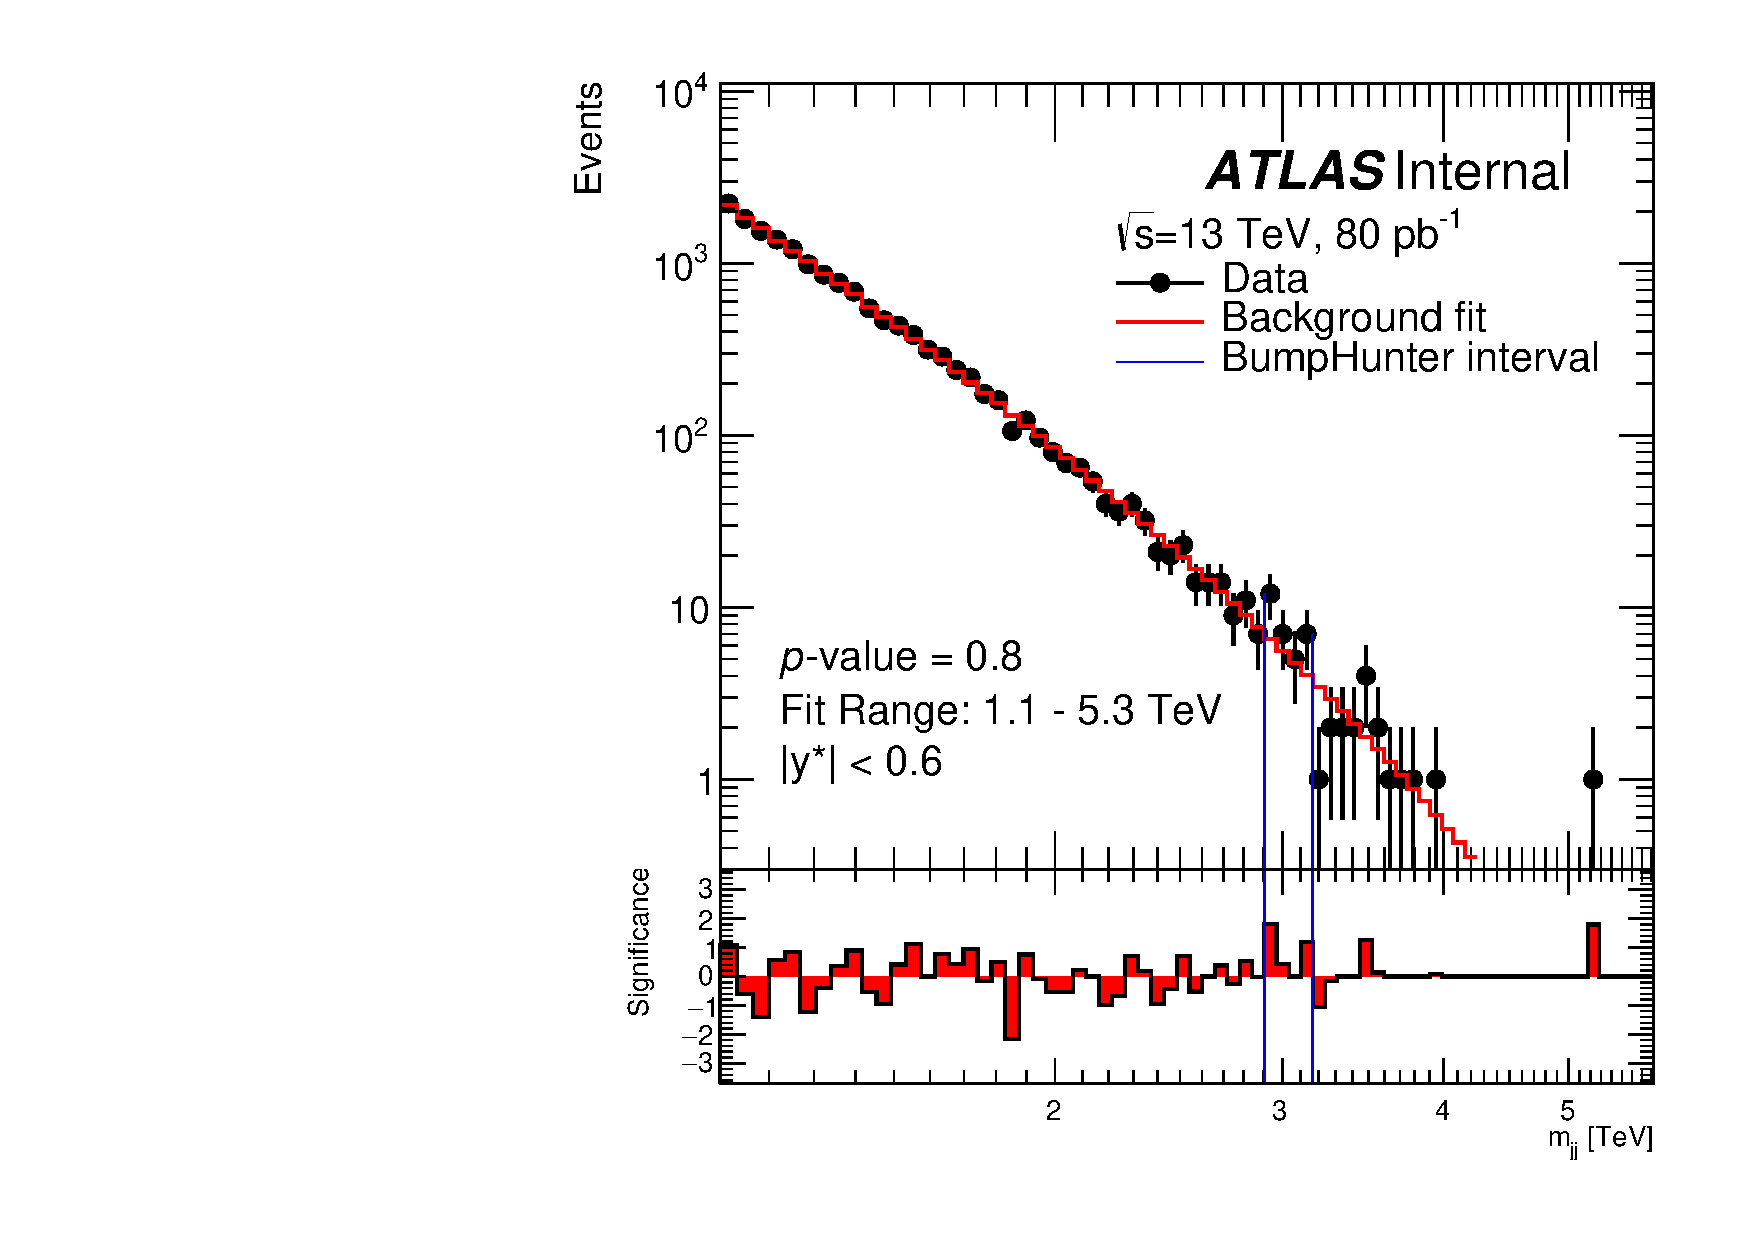
\includegraphics[scale=0.5]{LHCPplots/SearchPhase/figure1.pdf}
  \caption{figure1.pdf}
\end{figure}

\begin{figure}[htbp]
  \centering
  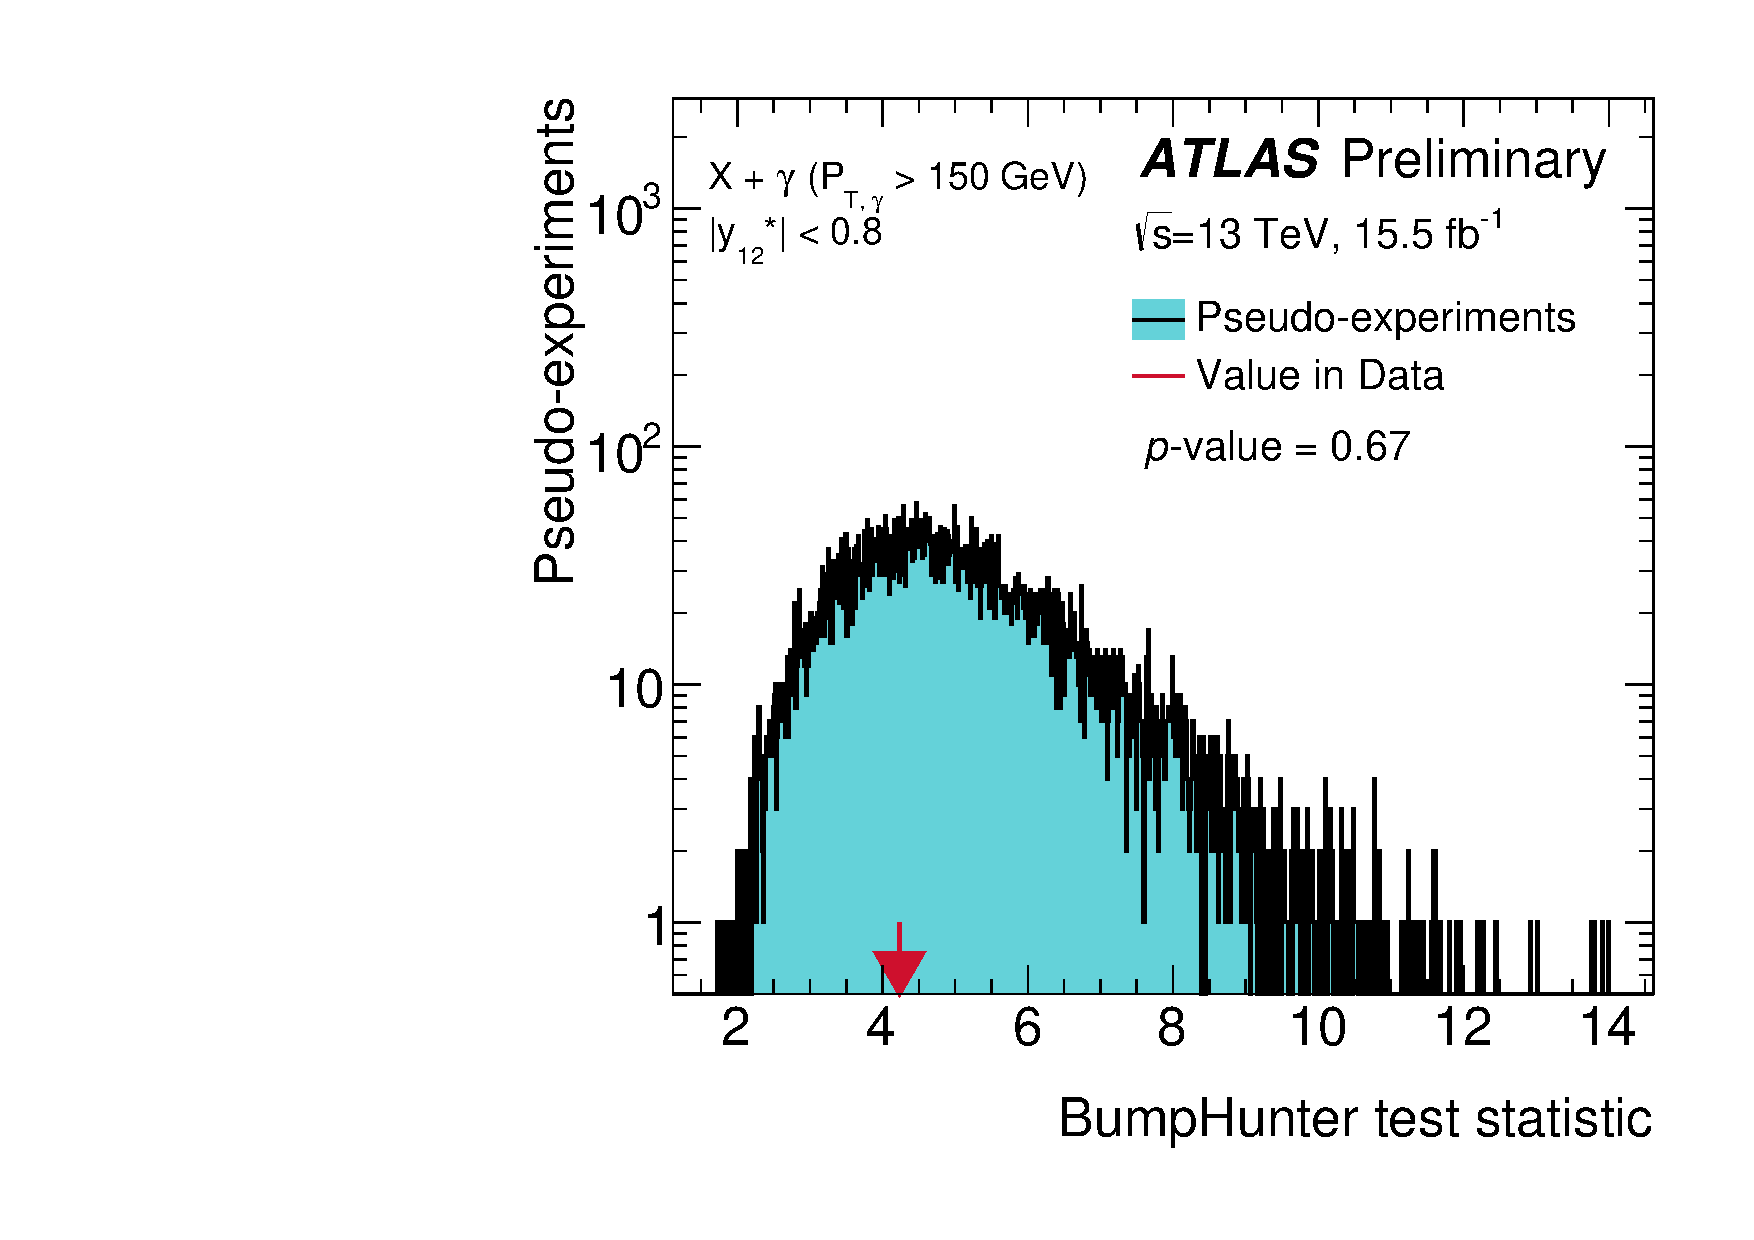
\includegraphics[scale=0.5]{LHCPplots/SearchPhase/bumpHunterStatPlot.pdf}
  \caption{bumpHunterStatPlot.pdf}
\end{figure}

\begin{figure}[htbp]
  \centering
  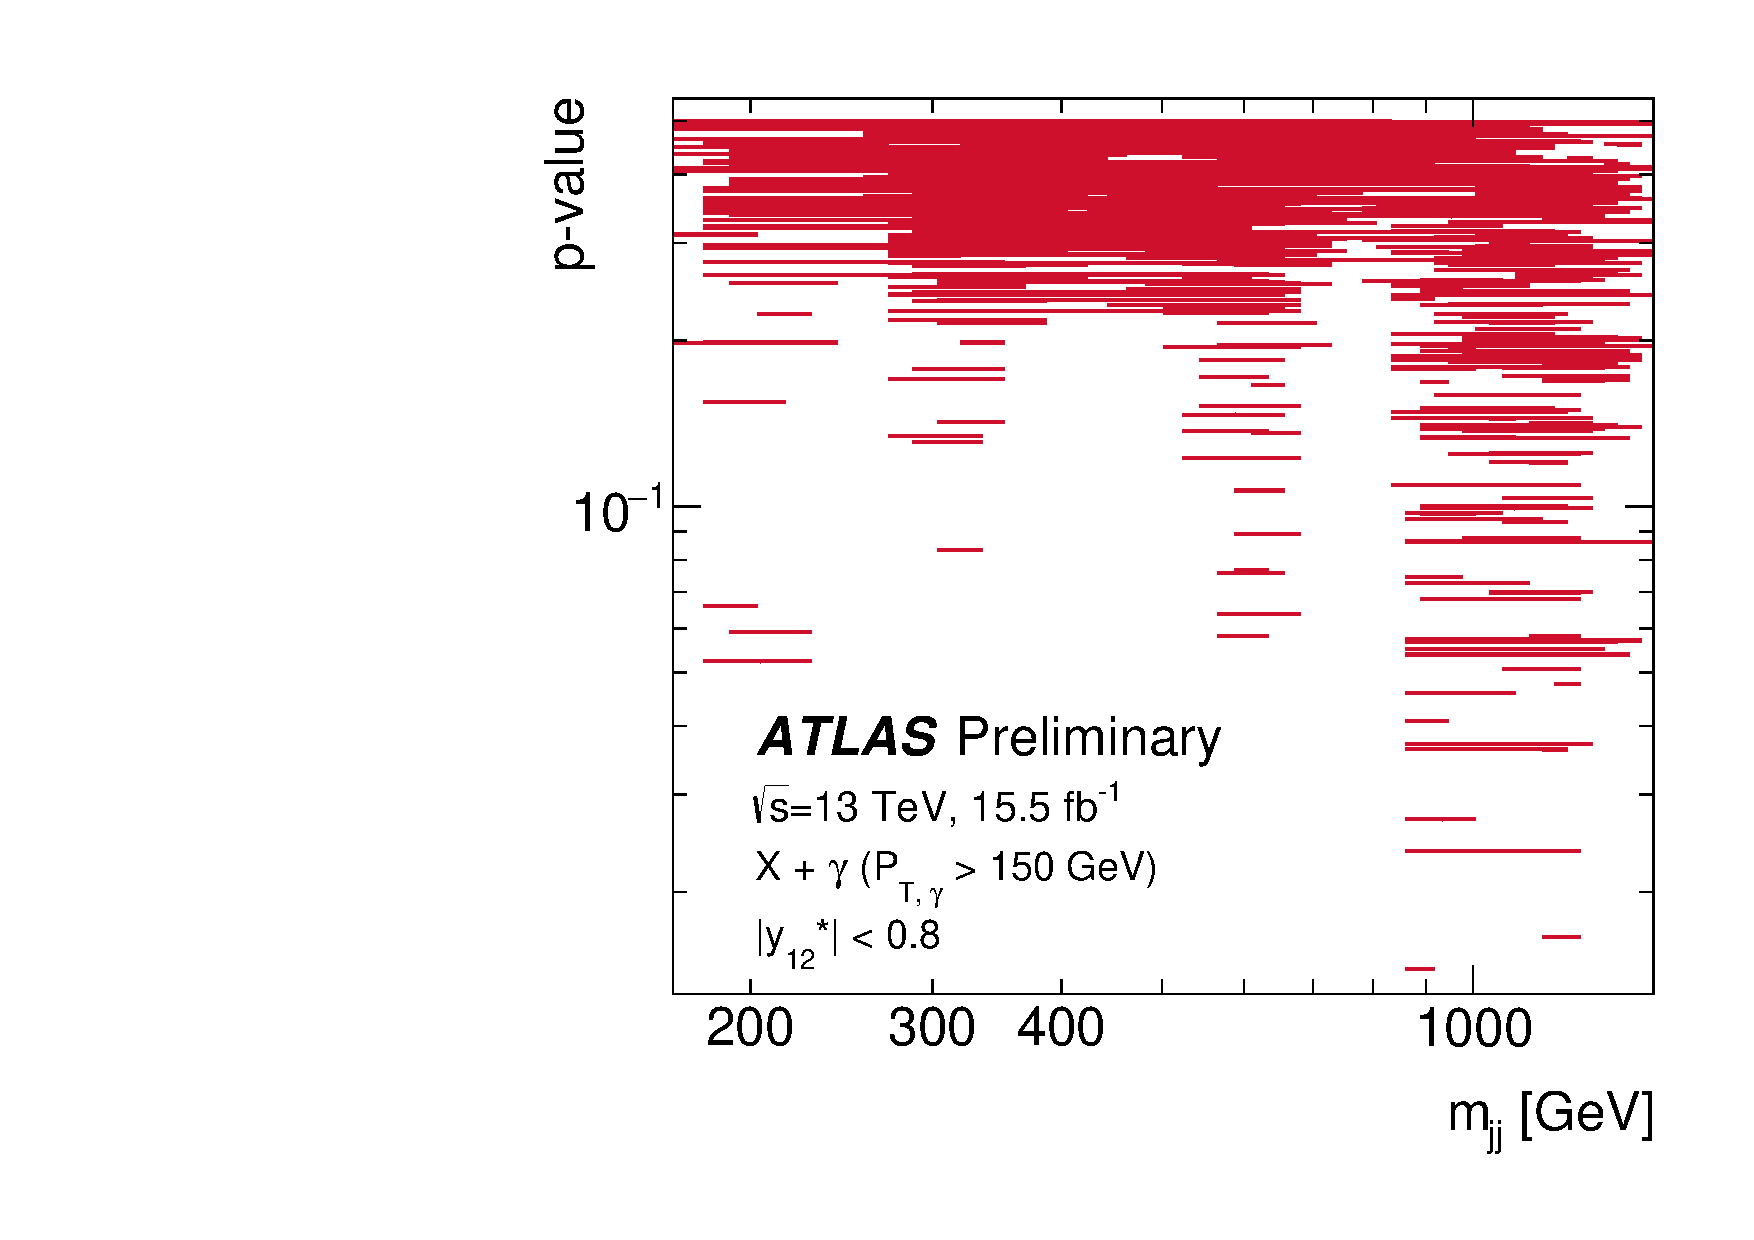
\includegraphics[scale=0.5]{LHCPplots/SearchPhase/bumpHunterTomographyPlot.pdf}
  \caption{bumpHunterTomographyPlot.pdf}
\end{figure}

\begin{figure}[htbp]
  \centering
  \includegraphics[scale=0.5]{LHCPplots/SearchPhase/{compareFitQualityAndFitChoice_Asymm_WithRatioPaper}.pdf}
  \caption{compareFitQualityAndFitChoice\_Asymm\_WithRatioPaper.pdf}
\end{figure}

\newpage

%-------------------------------------------------------------------------------
\subsection{Limit setting plots}
\label{subsec:limplots}
%-------------------------------------------------------------------------------

Paper values for comparison:

Bump low, high edges are 2905.0 3167.0\\\vspace{0.2cm}

Signal QStar\\
Observed limit at 95\% CL: 3.2\\
Expected limit at 95\% CL: 3.3 \\\vspace{0.2cm}

Signal BlackMax\\
Observed limit at 95\% CL: 6.5\\
Expected limit at 95\% CL: 6.6\\\vspace{0.2cm}

Second signal curve: QBH\\
Observed limit from this plot: 6.7\\
Expected limit from this plot: 6.8\\\vspace{0.2cm}

\begin{figure}[htbp]
  \centering
  \includegraphics[scale=0.5]{LHCPplots/LimitSetting/{FancyFigure1ExtendedWithFitLabels_QStar}.pdf}
  \caption{FancyFigure1\_QStar}
\end{figure}

\begin{figure}[htbp]
  \centering
  \includegraphics[scale=0.5]{LHCPplots/LimitSetting/{Limits_QStar}.pdf}
  \caption{Limits\_QStar.pdf}
\end{figure}

\begin{figure}[htbp]
  \centering
  \includegraphics[scale=0.5]{LHCPplots/LimitSetting/{FancyFigure1ExtendedWithFitLabels_QBH}.pdf}
  \caption{FancyFigure1\_QStar}
\end{figure}

\begin{figure}[htbp]
  \centering
  \includegraphics[scale=0.5]{LHCPplots/LimitSetting/{Limits_QBH_withBlackMax}.pdf}
  \caption{Limits\_QBH\_withBlackMax.pdf }
\end{figure}

\newpage


%-------------------------------------------------------------------------------
\section{Common mistakes}
\label{sec:mistakes}
%-------------------------------------------------------------------------------

Error message when plotting: 
\begin{lstlisting}[breaklines]
Tell ImportError: No module named art.morisot
\end{lstlisting}
You forgot to run the setup script to set the python path etc. Solution:
\begin{lstlisting}[breaklines]
. Setup.sh
\end{lstlisting}

\textcolor{red}{HERE onwards needs to be updated in the note!!}
%An annotated version of the configuration file which is used is included in appendix ~\ref{app:limitconfig}, and the output root files can be found in \verb results/QStar/JESTreatmentComparison  . Note that the \verb LimitSettingPhase_QStar_Reduced_splitJES_expected.config  file is used for mass points below $ \SI{1000}{\GeV}$ and \verb LimitSettingPhase_QStar_Reduced_1JES_expected.config  file is used for mass points above $ \SI{1000}{\GeV}$. 

%\item[Step 2] If the user wishes to only plot the observed and \textcolor{red}{expected limits}, without the error bands in order to do a quick test then consult appendix ~\ref{app:limitconfig}.

%\item[Step 3] In order to run over multiple mass points for a given signal sample the CERN batch system is used. \textbf{Important}: you must fill in the path to your package directory in the following file \verb setreducedlimits.sh  script in the \verb scripts  directory, i.e. replace \verb YYY  in the file. Once you have done this you can now run over four q* mass points by using the following command:
%\begin{verbatim}python calculateReducedLikelihoodsWithExp.py\end{verbatim} Currently there are only four mass points specified to be run over in \\\verb calculateReducedLikelihoodsWithExp.py , this is done in order to speed up the running time of the program for testing. If the user wishes to increase this number then the line \\\verb   signaldatasets['QStar'] = ['400','1250','2250','5250']  should be modified to include more mass points. The full set of mass points is displayed in the code under \verb # full mass points. Note that  \verb calculateReducedLikelihoodsWithExp.py  runs the the \verb setreducedlimits.sh  script. % where describe SED?
% \textcolor{red}{Note that this step currently takes approx 5 hours, I'm working on the best way to speed it up without making the test version more complicated!}

%  \item[Step 4] You can check on your batch jobs using the command \verb bjobs . Once the jobs are finished the output root files can be found in the \verb results/results/QStar/JESTreatmentComparison  folder. See appendix ~\ref{app:limitresults} for an explanation of each plot in \textcolor{red}{XXX}.

%\item [Step 5] In order to combine each of the output root files into \textcolor{red}{XXX} \verb LimitSettingPhase.cxx  must be run as follows:
%\begin{verbatim}LimitSettingPhase --config configurations/LimitSetting/ReducedCombinedLimitSetting_QS
%tar.config\end{verbatim} Note that if the number of mass points was modified in Step 2 then the \\\verb ReducedCombinedLimitSetting_QStar.config  file should be modified before running the above command. The modifications are as follows: \verb nMasses1  should be increased to the number of masses that you ran over in Step 2 and each of the mass points should be added to the list below that.

%\item [Step 6] In order to combine the plots in \verb likelihoodPoint_reduced_Slice0_YYY.root (where YYY is a given mass) into more meaningful plots \verb plotLimitSetting.py  in the \verb plotting  directory is used. To produce the plots do the following: 
%\begin{verbatim}cd plotting\end{verbatim}
%\begin{verbatim}python plotLimitSetting.py -b\end{verbatim}
%\end{description}
%\textcolor{red}{consistent directory/folderSAY ONLY USE QSTar and expl WHY e.g. configs, JES matrices etc.!here just expl calculateBayesian. Mention readme somewhere?

 %explain why it's necessary for them to add more mass points and more systematics etc to get a meaningful result.

%-------------------------------------------------------------------------------
\section{Examples of modifications that can be made to the code (search phase)}
\label{sec:examplessearch}
%-------------------------------------------------------------------------------
%\textcolor{red}{mention rc compile somewhere when update source code? or headers? do in making changes section? here or in limit setting section?}
%MjjHistogram(TH1F * inputHisto, string option, double thislumi)
%Constructor. option must be ”basic” or ”normalized”. If initialized using a basic TH1F, the normalized one is immediately created, and vice versa, so the MjjHistogram will always have both ”basic and ”normalized” histograms initialized. Third input is luminosity; this is stored as a property of the MjjHistogram and used for all normalization and unnormalization
%-------------------------------------------------------------------------------
\subsection{Selecting the range and initial fit function parameters for your mass spectrum}
\label{subsec:chooseparam}
%-------------------------------------------------------------------------------

The range (\verb minXForFit and \verb maxXForFit ) are specified in \verb SearchPhase.config as shown in appendix ~\ref{app:searchconfig}, and by default if these are set to -1 then the start and end of the data are used.  Note that only bins which fully contain the specified range are used e.g. if 1099 is specified for minXForFit then the next bin edge above this (e.g. 1100 GeV) is where the fit will begin from. 

\paragraph{} There is no definite way in which the  initial fit function parameters should be chosen, but some tips will be presented here. 
\begin{itemize}
\item As a starting point, \verb Parameters.txt  in the \verb configurations  directory provides some existing start parameters, so you can search for parameters for a sample with a luminosity similar to the one you are using.
\item  It should be noted that the first parameter for both the 3 and 4 parameter fit functions control the normalisation, so for example, the parameters for the 1 inv fb histograms could be used with the first parameter scaled to correspond to the luminosity you are using. 
\item If good start parameters are found for the 3 parameter fit, then the `alternative' fit (4 parameter function) the same initial start parameters as the 3 parameter function can be used, with the following two changes, parameter 3 should be set to the negative value of what was used for the 3 parameter fit (due to the way the 3 and 4 parameter functions are defined) and parameter 4 should be set to 0. 
\item If reasonable start parameters are found then run the search phase once to obtain the parameter values after fitting. These should be used as your new initial start paramters in the future (for this sample).
\end{itemize}

%\textcolor{red}{Mention selection of middle of bin, see book! step size? adjust? }
%259


%#maxXForFit       use default: maximum of data

%# Fit function parameters
%#nParameters	  5
%parameter1	  0.5
%parameter2	  7.5
%parameter3	  5.0
%parameter4	  0.15
%#parameter5	  6000

%\textcolor{red}{Show error message? When stop iterations, when within step size, explain where fitting is done and initial ROOT fit etc?}
%\textcolor{red}{Make fitting script to show users their chosen fit visually! then document it here}

%-------------------------------------------------------------------------------
\subsection{Using a different fit function}
\label{subsec:difffit}
%-------------------------------------------------------------------------------

%-------------------------------------------------------------------------------
\section{Examples of modifications that can be made to the code (limit setting phase)}
\label{sec:exampleslimit}
%-------------------------------------------------------------------------------
Adding in mass points and signals. 
If the user wishes to add another signal, other than QStar, then a new configuration file should be made e.g. \verb Step2_setLimitsOneMassPoint_WStar.config, where WStar is the name chosen by the user, and in \verb Run_Limits.py this signal and it's mass points should be added to the Signals dictionary, in the same way as for QStar, but using the name chosen by the user, e.g. WStar. 
%-------------------------------------------------------------------------------
\section{Search phase explanation}
\label{sec:searchexpl}
%-------------------------------------------------------------------------------
The aim of the search phase is to establish whether there are any statistically significant %explain!
excesses present in the measured dijet invariant mass spectrum. In order to do this the expected background from Standard Model particles, our  \textit{background only hypothesis}, is determined by fitting the spectrum with a smooth function. The function is chosen such that it does not accommodate the type of deviations which would be introduced by a resonance \textcolor{red}{reference paper or write about it}. The fitting procedure is described in more detail in section Section~\ref{subsec:smoothfit}. %\textcolor{red}{how test this?} %This method is data-driven, and avoids using Monte Carlo to model the background as this would introduce large theoretical uncertainties.

Once the fit has been performed, the resulting background only hypothesis is compared to our spectrum using a \textit{test statistic}.  A test statistic is used as this provides us with a single value which increases \textcolor{red}{monotonically} with decreasing compatibility, giving us a way to quantify the compatibility between our spectrum and the hypothesis. A variety of test statistics are available for analysers to use, and these are discussed in more detail in section ~\ref{subsec:teststat}.

 By calculating the \textit{p-value} \textcolor{red}{ref} of a test statistic we answer the question “What is the probability of observing data at least as extreme as the measured spectrum, given that the Standard Model is true?”, and we can reject the background only hypothesis if the p-value is lower than an agreed cutoff value.  The rejection of the background only hypothesis would indicate that the hypothesis is not sufficient to describe the data and may point to new physics. %\textcolor{red}{describe pval mathematically, average pval? small large pval significance?}
An explanation about how this is implemented in the code is provided in section ~\ref{subsec:pval}  . A more 
practical discussion about the inputs to the code and the weighting of events in our spectrum will now be presented. \textcolor{red}{mention/expl freq vs bayesian and freq search phase and bayesian limit setting, and why? LOOK http://arxiv.org/pdf/1101.0390v2.pdf !!!!!!}
%In the frequentist approach, a mathematical representation of this statement is given by the following formula: 
%\begin{equation}{P(x\in\omega|H)\leq\alpha}\end{equation},
%where the probability of obtaining our measured spectrum, \verb x  is one of the possible outcomes, $\omega$, that 

% A frequentist \textcolor{red}{method/approach} is employed for the search phase, and  %as we are investigating the probability of obtaining a certain outcome (our measured dijet invariant mass spectrum) given a certain hypothesis (the Standard Model).
%ok/expl more SEE and ref: https://svnweb.cern.ch/trac/atlasphys/browser/Physics/Exotic/Analysis/Dijet/Papers/DijetMassResonancesBackupICHEP2014/DijetResonancesBackup2013.pdf
%An explanation about how this is implemented in the code will now be provided.

%-------------------------------------------------------------------------------
\subsection{Search phase inputs and weighting}
%-------------------------------------------------------------------------------
The input to the search phase is a root Ntuple containing a dijet invariant mass spectrum after analysis selection and the \verb SearchPhase.config  configuration file which is described in appendix ~\ref{app:searchconfig}. The main file which performs the search phase is the \verb SearchPhase.cxx  file in the \verb util  directory. This file starts off by reading in the information from the configuration file and accessing the input Ntuple which contains the dijet invariant mass spectrum. 

If the input dijet invariant mass spectrum was produced using of multiple triggers with different prescales, then the spectrum will contain weighted events and the contents of a bin may be substantially different from the number of raw events that were used to fill it. In order to retain information at both levels, both at the weighted level and at the level of the raw events, the dijet invariant mass spectrum contained in the Ntuple is passed to the class \verb MjjHistogram, and an instance of this class called \verb theHistogram  is then created. The source file for \verb MjjHistogram  is in the \verb Root  directory and the corresponding header file is in the lower level \verb Bayesian  directory. 

The \verb MjjHistogram  class is a wrapper and contains three key histograms, which were produced from the input dijet invariant mass spectrum.  These histograms are as follows:
\begin{itemize}
\item The basic data histogram i.e. the weighted dijet invariant mass spectrum. 
\item The effective histogram, which has a value in each bin equal to the equivalent statistical power of the events in that bin in the basic histogram. \textcolor{red}{explain more and explain how calculated!}
\item The weights histogram, which has a value in each bin equal to the effective weight of each event in that bin in the effective histogram, and is used to convert between basic and effective histograms.
\end{itemize} \textcolor{red}{explain where each used? and how calc eff histo and weights}
Throughout the code \verb theHistogram  is used and is passed to all user-accessible functions such that the correct form can be accessed by the program. All comparisons between the observed spectrum and a hypothesis makes use of the effective statistics in the observed spectrum and an appropriately scaled version of the hypothesis, unless otherwise stated.  %clear? without the user needing to know which is required in a given situation. 
\textcolor{red}{stat uncerts! expl weighting below above 1TeV?}.

%-------------------------------------------------------------------------------
\subsection{Fitting a smooth function to the data}
\label{subsec:smoothfit}
%-------------------------------------------------------------------------------

%The fit and search strategy are described in detail in Section 8.
%The analysis technique and its sensitivity to given benchmark models are tested on simulated data prior to running the analysis code on ATLAS data. Further tests are provided by only analysing a partial dataset, meaning that the entire dataset was not analysed until the full set of event and object selection cuts is finalized. This strategy is complementary to blinding the signal region, when the background estimations is purely derived from data. It allows performance issues to be disentangled from the appearance of a signal: using a partial dataset limits the risk of a bias in the selection. The validation and sensitivity studies are described in Sections 9 and 10 respectively.
%The results of the search phase on the full 2012 dataset are presented in Section 11

The background is parameterised by fitting a smooth functional form to the observed dijet invariant mass spectrum. In the $\SI{8}{\TeV}$  dijet resonance a four parameter fit function that was chosen, and it has the following form:
 \textcolor{red}{XXX use equation mode}

where x \textcolor{red}{XXX}
 s is the ratio of the dijet invariant mass to the center of mass
energy and the p i are free parameters. The number of parameters and their default values are read in from the \verb SearchPhase.config  file and they are pushed back into the \verb paramDefaults  vector. The starting point for the fit \verb minXForFit  is also read in from the configuration file, and is stored as \verb minX in. The fit picks the low edge of the bin that contains the position \verb minXForFit   and fits down to that value.
 If \verb minXForFit  is within a bin that is below the first bin with data then \verb minX is reset to the first bin with data in the code. If \verb maxXForFit  is not specified in the configuration file then the end of the data is used instead.

The next step is to pass these values to the fit function. In order to do this an instance of the class 
\verb FourParamFitFunction  is created called \verb theMjjFitFunction which takes in the inputs \verb minXForFit, maxXForFit and Ecm, which are defined in the \verb SearchPhase.config  file. \verb FourParamFitFunction  is \textcolor{red}{defined} in the \verb MjjFitFunction.h  file in the lower level \verb Bayesian  directory, and this is where the fit functions are defined. For more information about creating your own fit fuction refer to section \textcolor{red}{ XXX. All fits that are created are daughter classes of the class  }\verb MjjFitFunction \textcolor{red}{ which is defined in the files XXX ..}

%-------------------------------------------------------------------------------
\subsection{Available test statistics}
\label{subsec:teststat}
%-------------------------------------------------------------------------------

Now the fit has been performed, we have a background hypothesis which we can compare to the observed spectrum. As mentioned in section ~\ref{sec:searchexpl}, a test statistic is used in order to quantify the compatibility between the hypothesis and the observed spectra, as it provides us with a single value which increases \textcolor{red}{monotonically} with decreasing compatibility. Three different values are used as test statistics in the search phase. 

%-------------------------------------------------------------------------------
\subsubsection{The BumpHunter}
\label{subsubsec:bumphunter}
%-------------------------------------------------------------------------------

The first statistical test which is created in \verb SearchPhase.cxx  is the BumpHunter \textcolor{red}{ref}, via the line:
\\\verb MjjBumpHunter  \verb theBumpHunter;  \\\verb theBumpHunter  is an instance of the class \verb MjjBumpHunter, which is defined in \verb MjjBumpHunter.cxx  in the \verb Root  directory, with it's corresponding header file in the lower level \verb Bayesian  directory. The BumpHunter starts with a two bin-window, set by the line \verb theBumpHunter.SetMinBumpWidth(2); , and it shifts its location such that all two bin-windows (i.e. neighbouring two bins) have been tested. The size of the window is then increased by one bin and the process is repeated, this continues until the bin-window range is half the number of bins in the full observed spectrum \textcolor{red}{where max bin range set?}.


 %In PAPER The most significant departure from the smooth spectrum (“bump”) is defined by the set of bins that have the smallest probability of arising from a background fluctuation assuming Poisson statistics. The BumpHunter algorithm accounts for the so-called “look-elsewhere eect” [47], by performing a series of pseudo-experiments drawn from the background estimate to determine the probability that random fluctuations in the background-only hypothesis would create an excess anywhere in the spectrum atleast as significant as the one observed. Furthermore, to prevent any NP signal from biasing the background estimate, if the most significant local excess from the background fit has a p-value smaller than 0.01, this region is excluded and a new background fit is performed. The exclusion is then progressively widened bin by bin until the p-value of the remaining fitted region is acceptable. The BumpHunter algorithm is detailed further in Section 8.2. This algorithm is dependent on the dijet mass resonance binning: the choice of binning is detailed in Section 8.3. The treatment of weighted data due to the trigger prescale weights is described in Section 8.5 Three different values are used as test statistics in the search phase to quantify the level of agreement between an observation and a spectrum serving as a hypothesis. These test statistics return a single value which characterises the entire spectrum and which increases monotonically with increasing discrepancy between observation and prediction, making them useful for defining p-values.
%-------------------------------------------------------------------------------
\subsection{p-value determination}
\label{subsec:pval}
%-------------------------------------------------------------------------------

\textcolor{red}{show these plots or final paper ones OR ones from reduced code and compare to paper!!!! locations in code? refer to change fit function section? }
\begin{figure}[htbp]
  \centering
  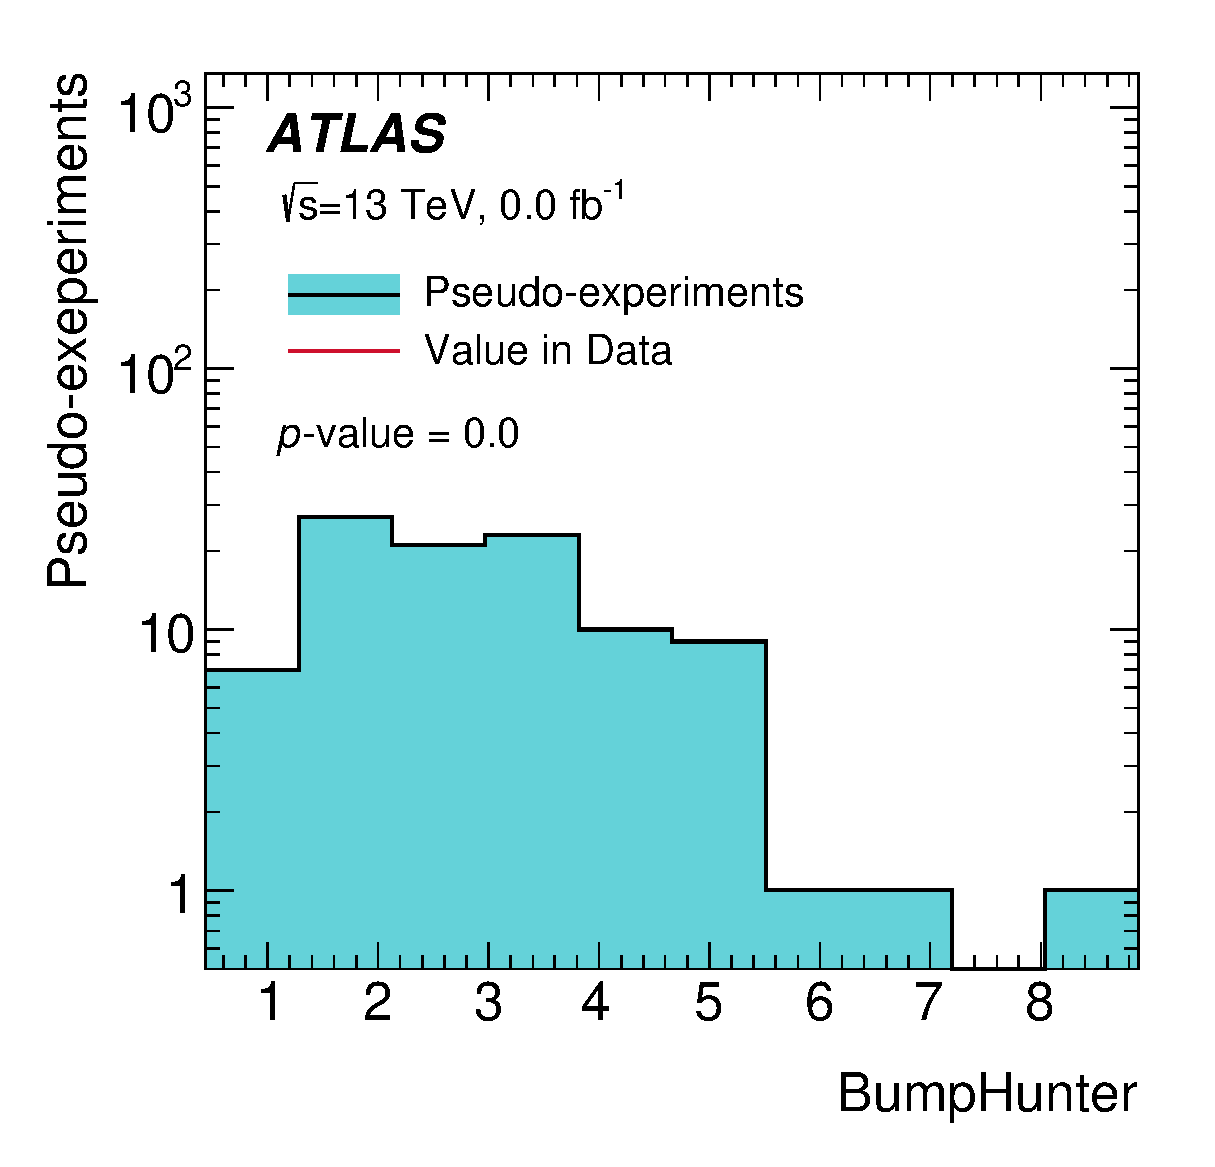
\includegraphics[scale=0.5]{myplots/bumpHunterStatPlot.eps}
  \caption{An example ATLAS figure2 UPDATE TO REDUCED VERSIONchange lumi etc and labels.}
  \label{fig:example2}
\end{figure}
\textcolor{red}{put other test statistic p val plots in appendix?}

%-------------------------------------------------------------------------------
\subsection{Representing significance bin-by-bin}
\label{subsec:significance}
%-------------------------------------------------------------------------------

%-------------------------------------------------------------------------------
\subsection{The resulting background only hypothesis}
\label{subsec:bkgonly}
%-------------------------------------------------------------------------------

\begin{figure}[htbp]
 \centering
  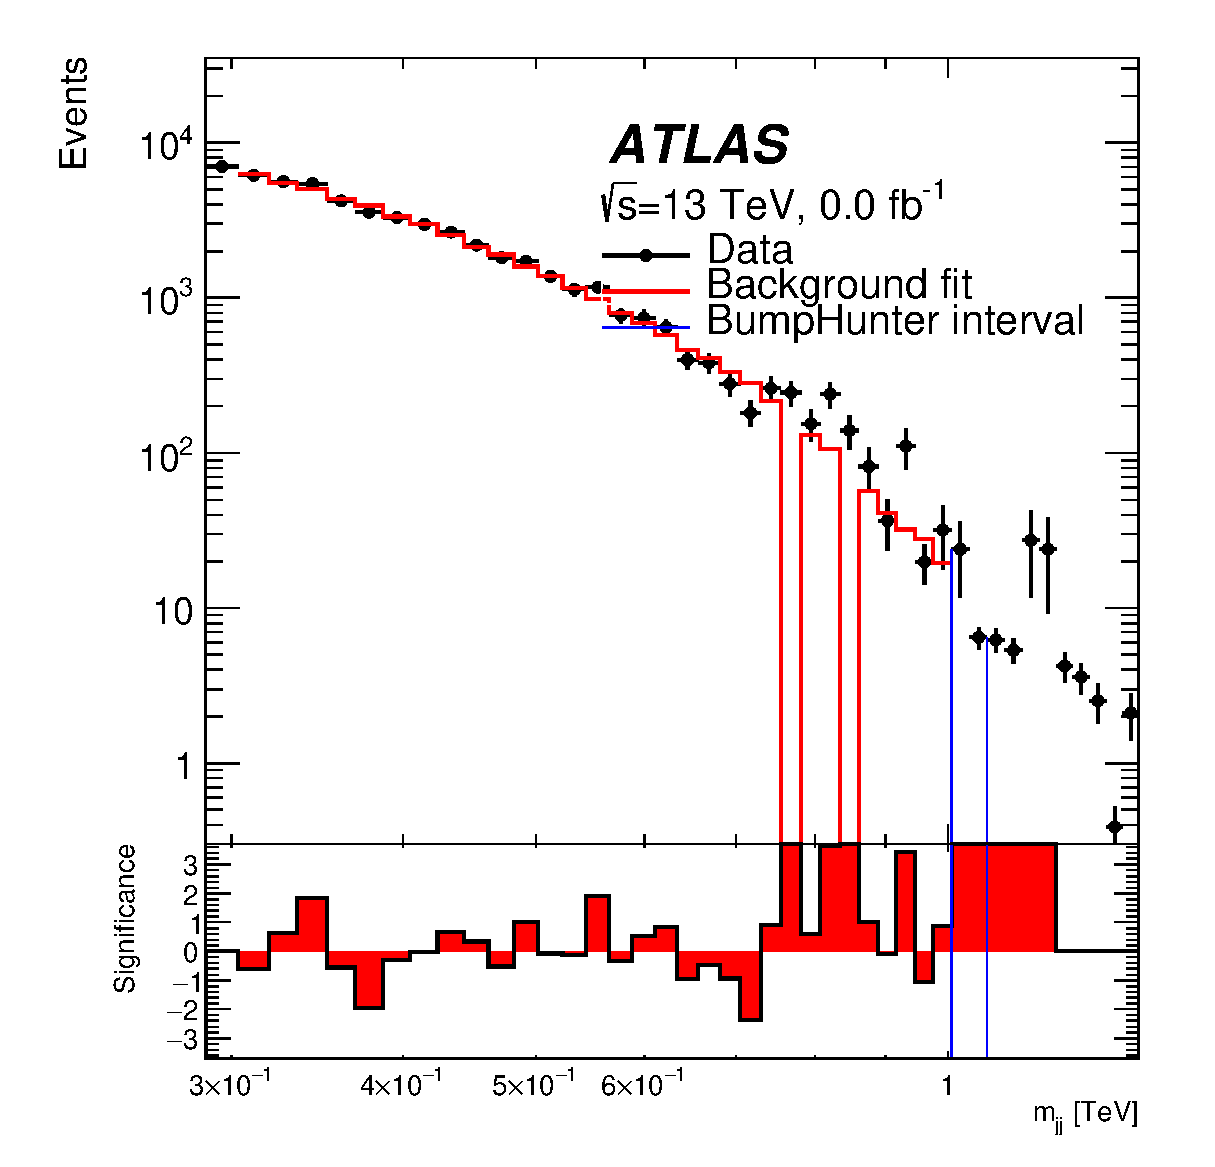
\includegraphics[scale=0.5]{myplots/figure1.eps}
  \caption{An example ATLAS figure. UPDATE TO REDUCED VERSION. change lumi etc and labels!}
  \label{fig:example}
\end{figure}

%-------------------------------------------------------------------------------
\section{Limit setting phase explanation}
\label{sec:limitexpl}
%-------------------------------------------------------------------------------
In the case that there is no statistically significant excess found in the dijet invariant mass spectrum, then the limit setting phase is performed. This phase is carried out in order to set limits on the rate of production of a new particle \textcolor{red}{ or process}. Each new particle that is considered is described by a particular model, which describes the shape of the resonance the presence of this particle would create, and also the cross section for the production of this particle for given particle masses. When setting limits on this new particle \textcolor{red}{or process}, the question that we ask for each particle mass is as follows; "What is the probability %\textcolor{red}{With 95\% certainty NO? could} 
that this particle with this mass exists, given our observed data". In order to answer this question an upper limit on the number of `new particle events' that could be contained in the data is determined. This upper limit is then converted into the maximum allowed cross-section for the new particle at each mass. \textcolor{red}{interpolate?} The intersection between this `observed' limit and the nominal cross-section for the new particle \textcolor{red}{or process} gives the highest mass of this new particle that we can exclude \textcolor{red}{95 percent level?}. The details of the limit setting are described below, together with references to where each step is carried out in the code.  %\textcolor{red}{\\$\sqrt{s} = \SI{8}{\TeV}$ results too? CAREFUL cross sec x acceptance, recap!!!!!!!! mention falling xsec higher m? less ev, think signal grow higher rate than bkg once above threshold i.e. a lot higher than M new particle due to PDFs?bayesian vs freq, nuisance etc?think mass vs rate or equiv in this case? think why flat prior bayes not like frequentist? overload prior? Ask 3 lines limit obs exp and q* check we use intersection obs and exp? why incl q* and not match expected? incl change lumi blinded unblinded, make clean disconnect eos, incl 1 2 bit: Well the good thing is in our case it's only ever 1 or 2. The issue is that BAT internally keeps track of all parameters by the order you add them to the model you build. My code adds all the background-related nuisance parameters first, and then all the signal-related ones. But there are only ever 1 or 2 background ones for us, meaning that the signal normalisation (our parameter of interest) is either the 2nd or 3rd parameter to get added to the model. We could rearrange it and always make that one first or something but this is just how I set it up the first time and I didn't see any point in messing with it. You can if you want though! it's all in setLimitsOneMassPoint.} \textcolor{red}{ what is 'expected' limit and bands used for?}

% Having all the mass points is really important if you want this to have physical meaning because that is how we get any sort of precise look at the limits. the step from running a mass point to putting together the plot is really easy -- just divide points by luminosity and graph them




% All figures and tables should appear before the summary and conclusion
% The package placeins provides the macro \FloatBarrier to achieve this
% \FloatBarrier

%-------------------------------------------------------------------------------
\section{Summary and conclusion}
\label{sec:summary}
%-------------------------------------------------------------------------------


%Please make sure that there is a conclusion! The concluding statements should reflect what is in the abstract. Reiterate the main points of the paper and the primary results and conclusions.

%Note that many readers look mostly at the title, abstract and conclusion. The conclusion should be interesting enough to make them want to read the whole paper. It is not good style just to repeat the abstract. If your paper is short and only has one result quoted at the end of the paper, then you should consider whether conclusions are necessary.

%Try not to end your conclusions with a sentence such as ``All the results in this paper are in good agreement with the Standard Model, the current world average and recent measurements by other experiments.''  This might lead a referee (internal or external) to wonder why it is worth publishing this paper!

%Note that all figures and tables should be output before the start of the ``Summary and conclusion''. This can be achieved using the macro \Macro{FloatBarrier} that is part of the \texttt{placeins} package.

%-------------------------------------------------------------------------------
\section*{Acknowledgements}
\label{sec:acknowldge}
%-------------------------------------------------------------------------------

%A standard template for the acknowledgements is available on the web pages of the Publication Committee. See reference~\cite{publication-policy} for the URL. The acknowledgements should be in an unnumbered section.


%-------------------------------------------------------------------------------
% Bibliography
%-------------------------------------------------------------------------------
\printbibliography
% This document uses biblatext and bib to process the bibliography.
% If you want to use BibTeX you need to use the syntax below.
% \bibliographystyle{../atlasBibStyleWoTitle}
% \bibliography{BayesianNote}


%-------------------------------------------------------------------------------
\newpage
\appendix
\part*{Appendices}
\addcontentsline{toc}{part}{Appendices}
%-------------------------------------------------------------------------------

%In general, you use the appendices to include all the technical details of your work that are relevant for the ATLAS Collaboration only (e.g.\ dataset details, software release used). In an ATLAS paper auxiliary plots and tables that are supposed to be made public should be collected in an appendix.

%-------------------------------------------------------------------------------
\section{Provided inputs to the code}
\label{app:inputs}
%-------------------------------------------------------------------------------
\begin{itemize}
\item \verb Data15_C_fGRL_JetCalibCorrection_20150721/dataHistograms.PeriodC.root: The input Ntuple to the code, which contains the dijet invariant mass histogram after analysis cuts.
\item \verb  xsecandacceptance :  Directory containing  CrossSectionsFor13Plotting.root  and Templates\_QStarQBH\_1fb.root .  The former contains the theory line for the limit plot and the latter contains the signal templates used for the `Fancy\_Figure' plots of the mjj spectrum with overlaid signal bumps.
\end{itemize}
%-------------------------------------------------------------------------------
\section{Step1\_SearchPhase.config }
\label{app:searchconfig}
%-------------------------------------------------------------------------------

\begin{verbatim}
##############################################
#                                            #
#  Config file for Bayesian                  #
#                                            #
##############################################

#set all the parameters of your analysis
#IMPORTANT: don't leave spaces after the parameters!

	
##########################################
# input/output
##########################################

# This contains the data spectrum which will be analysed
# Value overwritten if use Run_SearchPhase.py
inputFileName ./inputs/Data15_C_fGRL_JetCalibCorrection_20150721/dataHistograms.PeriodC.root

# Value overwritten if use Run_SearchPhase.py
dataHist Nominal/mjj_Data_PeriodC_0p072fb

# Value overwritten if use Run_SearchPhase.py
outputFileName ./results/Step1_SearchPhase/Data15_C_fGRL_JetCalibCorrection_20150721/Step1_SearchPhase_mjj_Data_PeriodC_0p072fb.root

##########################################
# general
##########################################

# Center-of-mass energy of the spectrum studied
# Value overwritten if use Run_SearchPhase.py
Ecm        13000.0 

# Number of pseudoexperiments to run
# Matches 8 TeV paper value
nPseudoExp 10000

##########################################
# fitting
##########################################

# To use min of data put -1 (Use 1099 so fit starts from bin above, i.e. from 1100 GeV)
minXForFit       1099 

# use default: maximum of data
maxXForFit       -1   

# 13 TeV 3 param fit function:
# this will be nominal function for now.
functionCode		9
nParameters 		3

# For Up to Period C4 data (72 inv pb)
parameter1   0.00307775 
parameter2   15.1199 
parameter3   -4.57371 

# 13 TeV 4 param fit function:
doAlternateFunction     true
alternateFunctionCode	4
alternateNParameters	4

# For Up to Period C4 data (72 inv pb)
altparameter1   69.3597
altparameter2   27.3806
altparameter3   -1.67095
altparameter4   -1.0643

doPValWithSysts		true

doPEOnData		false\end{verbatim}

Comments: If \verb outputFileName  is changed then it should be changed in the limit setting configuration files too as this file is an input to the limit setting phase. \textcolor{red}{expl nPseudoExp}  \verb minXForFit  is the centre of bin value, but the fit actually picks the low edge of this bin and fits down to that value. \verb maxXForFit  is not specified as the end of the data is used instead. The fit function parameters are currently set up to be used with the four parameter fit function as described in section \textcolor{red}{XXX}. If the user wishes to switch to the five parameter fit function, also  described in section \textcolor{red}{XXX} then \verb nParameters  and \verb parameter5  should be uncommented, for further details about switching fit function see section \textcolor{red}{XXX}.



%\textcolor{red}{DO/update ->}Move all name change stuff e.g.  \verb SearchPhase\_results.root  (or alternative name specified in configuration file) to annotation in appendix folder also bit about changing  If an alternative name for \verb SearchPhase\_results.root  was specified in the configuration file then the \verb searchInputFile  value should be changed in  \textcolor{red}{why verb not work here?} plotter.py.

%-------------------------------------------------------------------------------
\section{Search phase results explanation}
\label{app:searchresults}
%-------------------------------------------------------------------------------
\verb SearchPhase_results.root  contains the following histograms:
\\\verb basicData: Input dijet invariant mass histogram
\\\verb normalizedData: Input dijet invariant mass histogram normalized by bin width \textcolor{red}{check and where used?}
\\\verb theFitFunction: The function fitted to the dijet invariant mass histogram
\\\verb basicBkgFrom4ParamFit: Same as theFitFunction, but in histogram form \textcolor{red}{ask/how decide binning, match original mjj binning?}
\\\verb normalizedBkgFrom4ParamFit: basicBkgFrom4ParamFit normalized by bin width
\\\verb residualHist: XXX
\\\verb relativeDiffHist: XXX
\\\verb sigOfDiffHist: XXX
\\\verb logLikelihoodStatHistNullCase: XXX
\\\verb logLOfFitToData: XXX
\\\verb bumpHunterStatHistNullCase: XXX
\\\verb bumpHunterStatOfFitToData: XXX
\\\verb bumpHunterTomographyFromPseudoexperiments: XXX
\\\verb bumpHunterPLowHigh: XXX
\\\verb fittedParameters: XXX
%-------------------------------------------------------------------------------
\section{Step2\_setLimitsOneMassPoint\_QStar.config}
\label{app:limitconfig}
%-------------------------------------------------------------------------------

\begin{verbatim} ##############################################
#                                            #
#  Config file for Bayesian                  #
#                                            #
##############################################

#set all the parameters of your analysis
#IMPORTANT: don't leave spaces after the parameters!

	
##########################################
# input/output
##########################################

# This input to limit setting phase must be an output from the search phase
# Value overwritten if use Run_SearchPhase.py
dataFileName ./results/Step1_SearchPhase/Data15_C_fGRL_JetCalibCorrection_20150721/Step1_SearchPhase_mjj_Data_PeriodC_0p072fb.root

dataHist          basicData

# Value overwritten if use Run_SearchPhase.py
signalFileName inputs/QBH_20150715/1fb/QBH%d_1fb.root

# Value overwritten if use Run_SearchPhase.py
nominalSignalHist mjj_QBH%d_1fb_Nominal

# Value overwritten if use Run_SearchPhase.py
outputFileName ./results/Step2_setLimitsOneMassPoint/Data15_C_fGRL_JetCalibCorrection_20150721/Step2_setLimitsOneMassPoint_QBH5000_0p072fb.root

# Put LogFiles in this folder
# Value overwritten if use Run_SearchPhase.py
plotDirectory .

# If you want to keep the BAT output plots with a distinguishable name, specify it here
plotNameExtension QStar

# Name of signal for retrievals etc
signame		  QStar

##########################################
# general
##########################################

# Value overwritten if use Run_SearchPhase.py
Ecm		  13000.0

minXForFit	  1099

nParameters       3

##########################################
# for limits
##########################################

nSigmas		  3.

doExpected	  true

# Lydia changed 10 to 100
nPEForExpected	  100

##########################################
# Background
##########################################

doFitError	  true

nFitsInBkgError	  100

##########################################
# Lumi
##########################################

doLumiError       true
# 9% lumi error
luminosityErr	  0.09

##########################################
# Function choice
##########################################

doFitFunctionChoiceError true

nFitFSigmas       1

alternateFunctionCode	4
alternateNParameters	4
# For Up to Period C4 data (72 inv pb)
altparameter1   69.3597
altparameter2   27.3806
altparameter3   -1.67095
altparameter4   -1.0643

##########################################
# Beam energy systematic
##########################################

doBeam		 false

BeamFile          ./inputs/BeamUncertainty/AbsoluteBEAMUncertaintiesForPlotting.root

##########################################
# JES
##########################################

doJES		  true

##--------------------------------------##

useMatrices       false

nominalJES         #matrix_mjj_TotalUncertainty_05

nComponents       1
name1		  1

##--------------------------------------##

useTemplates      true

# Value overwritten if use Run_SearchPhase.py
nominalTemplateJES mjj_QStar%d_1fb_Nominal

nComponentsTemp 3 
nameTemp1         mjj_QStar%d_1fb_JET_GroupedNP_1
nameTemp2         mjj_QStar%d_1fb_JET_GroupedNP_2
nameTemp3         mjj_QStar%d_1fb_JET_GroupedNP_3

##--------------------------------------##
# nJES is number of extensions +1 
nJES		  13
extension1        __3down
extension2        __2down5
extension3        __2down
extension4        __1down5
extension5        __1down
extension6        __0down5
extension7        __0up5
extension8        __1up
extension9        __1up5
extension10       __2up
extension11       __2up5
extension12       __3up
\end{verbatim}
%Comments: \textbf{Important}: Any changes made here must also be made in \verb LimitSettingPhase\_QStar\_Reduced\_1JES\_expected.config  as well, unless the changes are to the name or number of components of the JES uncertainty (i.e. modifying \verb nComponents  or \verb name1,2 ...  below \verb nComponents.  \\\textcolor{red}{put in comment signalFileName gives the location of the signal Monte Carlo file that we're setting limits on and nominalSignalHist mjj gives the name of the dijet invariant mass spectrum for this signal alone. The For more information about the inputs to the code stored in the DATA directory see appendix \ref{app:inputs}. }\textcolor{red}{explain plotDirectory,
%plotNameExtension,signame?}. 
%\\\verb minXForFit  is the centre of bin value, but the fit actually picks the low edge of this bin and fits down to that value. \verb maxXForFit  is not specified as the end of the data is used instead.\textcolor{red}{explain sigmas} 
%\\\\In order to \textbf{turn off the bands} on the limit plots to significantly speed up the running of the program, set \verb doExpected  to \verb false  in the \verb for  \verb limits section of the configuration file. 
%\\\\The number of pseudoexperiments than are run in order to \textcolor{red}{XXX}, \verb nPEForExpected  can be increased or decreased by changing the number. It should be noted that if too many pseudoexperiments are chosen then the program will take a long time to run, which is why this process is parallelised when producing the full paper results, for more information see section \textcolor{red}{XXX}. However; if too few pseudoexperiments are run then either no error bands will appear \textcolor{red}{check} or there will only be one error band \textcolor{red}{explain why}.
%\\\\
 Individual systematics can be turned on or off by changing e.g. \verb doFitError  from \verb  true  to  \verb false .% \textcolor{red}{explain where syst description is?} \textcolor{red}{explain difference splitJES and 1 JES and difference between this and paper config!!/merge into 1 and tell turn on?}

%-------------------------------------------------------------------------------
\section{Limit setting phase results expanation}
\label{app:limitresults}
%-------------------------------------------------------------------------------

%\begin{figure}[htbp]
%  \centering
%  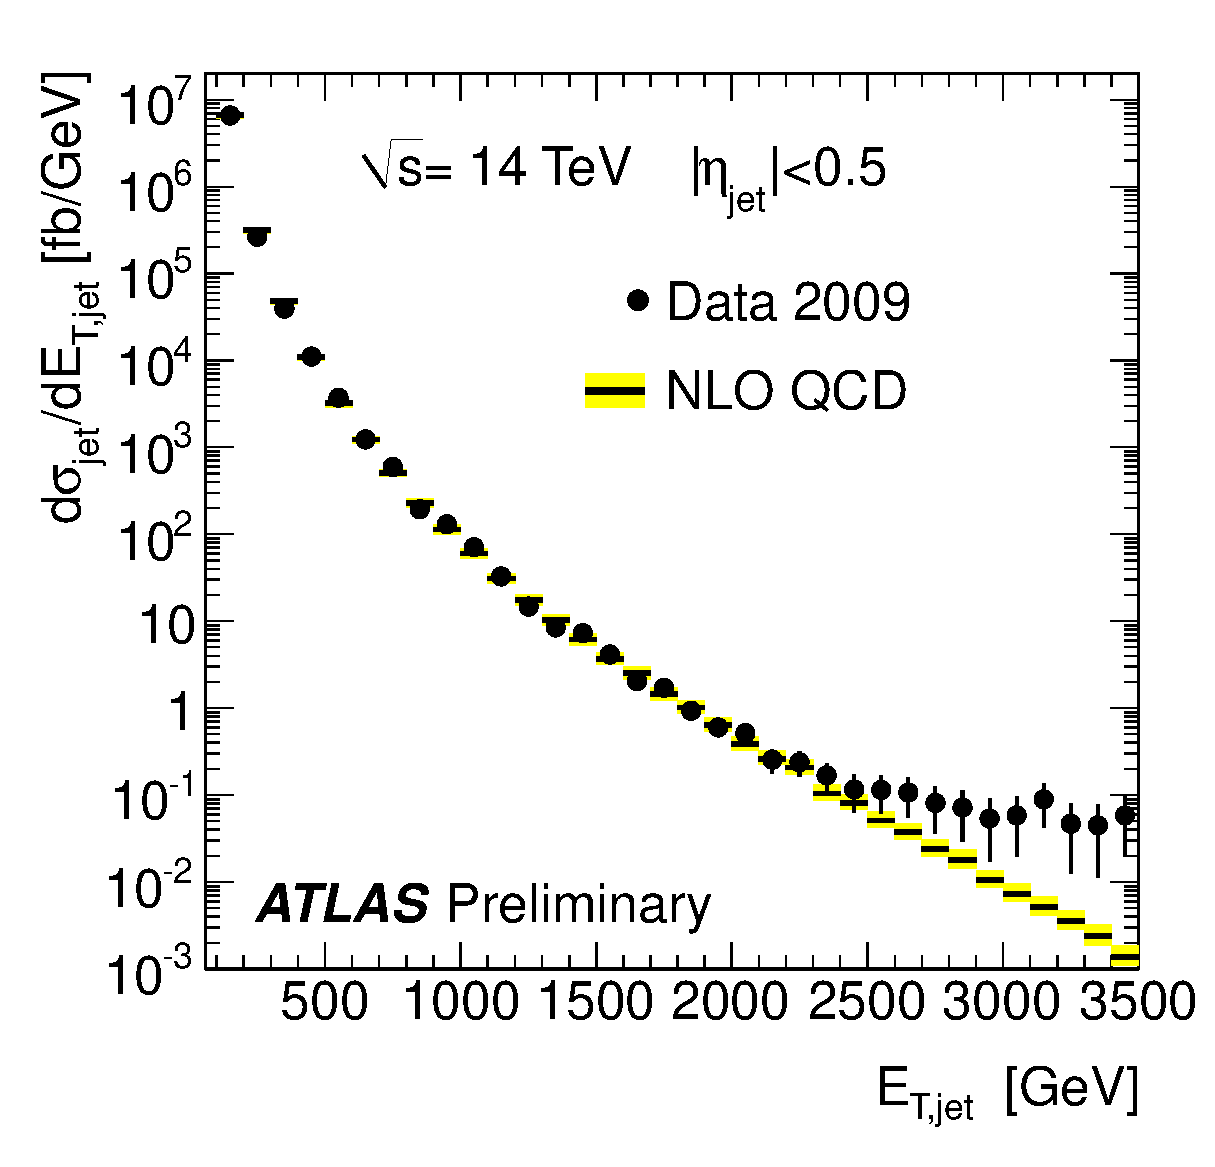
\includegraphics[width=\columnwidth]{AtlasExample}
%  \caption{An example ATLAS figure.}
%  \label{fig:example}
%\end{figure}

%Figures should be always made available in both %\texttt{eps} (or \texttt{pdf}) and 
%\texttt{png} format. Additionally, a \texttt{pdf} %version of the plots can be
%useful in case \verb|pdflatex| is used to produce a %publication.
%Colour versions are appropriate for talks, and black-%and-white
%versions are necessary for the publication itself.

%All figures appearing in the paper must be mentioned %in the text.
%The figures should appear in the same order as %mentioned in the text.
%At the beginning of a sentence, use the full word %``Figure''.
%Within a sentence, the abbreviation ``Fig.'' may be %used.
%If a figure appears in two or more parts, refer to it %as
%``Fig. 1(a)'' and ``Fig. 1(b)''. Both ``(a)'' and %``(b)'' should
%appear in the text, in the figure, and in the caption.
%The word ``ATLAS'' (or ``ATLAS Preliminary'', if %appropriate) should
%appear prominently somewhere in the figure. This %becomes important when
%the figure is copied and shown out of context. If %appropriate, it
%is useful to include information about the luminosity %corresponding
%to a figure.



%-------------------------------------------------------------------------------
\section{References}
\label{sec:refs}
%-------------------------------------------------------------------------------
%SEE REF SEC OF ORIGINAL DOCUMENT!


\end{document}
